\section{Results}

{{For a watertight shell model,}} both its inner and outer boundary need to be supported by a huge amount of materials in order to guarantee a fine surface quality. See Fig. \ref{fig:dear-simulation} (a-b) for an illustration of the Sculpture model, both its inner and outer surface require a significant amount of support in order not to be deformed during the printing process; while our approach only keeps all cylindrical shells that are free of support (Fig. \ref{fig:dear-simulation} (c-d)).

\begin{figure}[t]
  \centering
  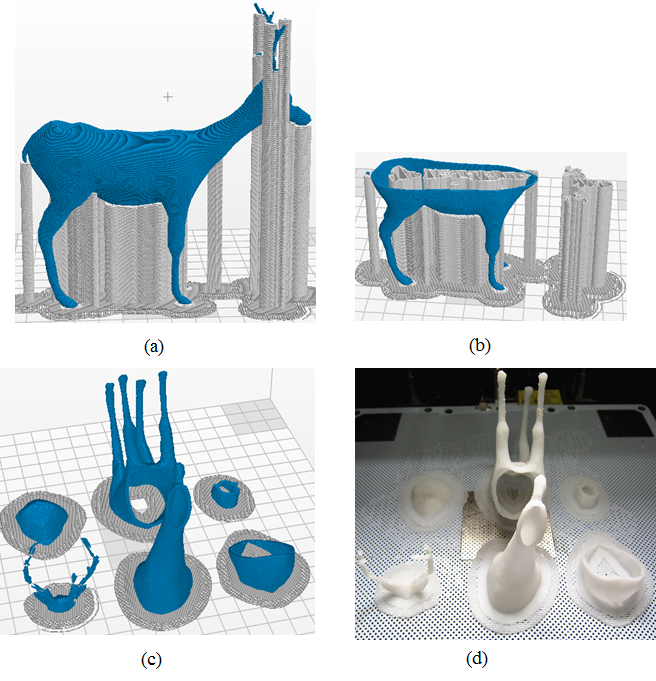
\includegraphics[width=\linewidth]{figs/dear-simulation.png}
  \caption{\label{fig:dear-simulation}%
           An illustration of the Sculpture model under the 3D printing software Z-suite as $\theta = 20^{\circ}$: (a) the full model; (b) an intermediate step of the simulation; (c) the simulation result of our partition for the Sculpture model; (d) the 3D printed result of our partition for the Sculpture model, no support is required except for the bed (limited by FDM technique).}
\end{figure}




We have run our algorithm on various natural and man-made models, and some of the results are presented in Fig. \ref{fig:experiment}. The left column of the figure exhibits the most material-saving orientation for printing the models using the Meshmixer software, a free software provided by Autodesk company. We validated our approach by a set of printing experiments on a Zortrax desktop printer, a kind of FDM machine that allows a printing layer thickness of 0.09mm, this is also the layer thickness we used in the printing experiments. The experiments are based on the choice of $\theta = 70^{\circ}$, i.e., all overhangs with an angle of no larger than $20^{\circ}$ with respect to the build platform are given support structures. Zortrax provides a built-in 3D printing software called \emph{Z-suite} that can automatically count the filament of the print material (in meters) and an estimate of the weight of the print material. Table \ref{tab:ertms:summary} summarizes the printing material and time that are consumed by the original models and our partitioned models. Our approach significantly reduces both the printing material and time as the skeleton-based partition reduces both the supported materials inside and outside the models.


\begin{table*}[htb]

\begin{footnotesize}

\begin{center}

    \begin{tabular}{p{1cm} p{1cm} p{1.7cm} p{1.7cm} p{1.4cm} p{1.4cm} p{1.5cm} p{1.5cm} p{1.3cm} p{1.3cm}p{1.4cm}}

    \hline

     Models& Skeleton generation time& Print material (original)& Print time (original)& Number of parts (skeleton partition)& Number of parts (mesh partition)& Print material (partition)& Print time (partition)& Material save (\%) &Time save(\%)\\ \hline
     Tree& 15.37s& 8.07m (19g)& 6h 9min &6 & 8 &5.19m(12g) & 4h 2min & 35.6877 &34.4173\\ \hline
     Armadillo& 82.54s& 7.7m (18g)& 5h 15min &9 & 10  &4.65m(11g) & 3h 30min & 39.6104 &33.3333\\ \hline
     Octopus& 6.72s& 14.31m (34g)& 10h 56min &5 & 9  &8.75m(21g) &6h 51min & 38.8539 &37.3476\\ \hline
     Deer& 11.42s& 10.52m (25g)& 8h 54min &4 & 6  &8.89m(21g) &5h 25min & 15.4943 &39.1386\\ \hline
     Airplane& 25.23s& 6.58m (16g)& 5h 42min &5 & 7 &5.24m(12g) &3h 10min & 20.3647 &44.4444\\ \hline
     Knots& 3.46s& 21.45m (51g)& 16h 41min &10 & 15 &12.38m(29g) &11h 20min & 42.2844 &32.0679\\ \hline
     Sculpture& 6.28s& 21.85m (52g)& 18h 41min &4 & 10 &16.35m(39g) &11h 23min & 25.1716 &39.0723\\ \hline
     Gargoyle& 55.34s& 6.75m (16g)& 5h 18min &4 & 5 &5.16m(12g) &3h 48min & 23.5556 &28.3019\\ \hline
     Bearing & 55.34s& 8.52m��20g�� & 6h 33min &10 & 10 &7.36m(18g) &4h 42min & 13.62 &28.24\\ \hline

    \end{tabular}

\end{center}

\end{footnotesize}

\caption{Statistics showing the print material, print time and partition number of the printed models.}\label{tab:ertms:summary}

\end{table*}


\begin{table*}[htb]

\begin{footnotesize}

\begin{center}

    \begin{tabular}{p{1.9cm} p{1.3cm} p{1.3cm} p{1.3cm} p{1.3cm} p{1.3cm} p{1.3cm} p{1.3cm}p{1.3cm}p{1.3cm}}

    \hline

     Models& Tree& Armadillo& Octopus& Deer& Airplane& Knots &Sculpture & Gargoyle & Bearing \\ \hline
     number of vertices & 11443   & 34594   & 1343    & 8917  & 15485 & 2904    & 5979    &25002 & 44945\\ \hline
     number of skeleton arcs    &130 & 143 & 81 &77 &60 & 77 &56  &50 &44\\ \hline
     time    &187.2576s & 346.374s & 102.1403s &93.6414s &91.8654s & 95.8742s &76.8461s  &202.7632s &173.4283\\
  \hline

    \end{tabular}

\end{center}

\end{footnotesize}

\caption{The running time of processing the models with our stochastic algorithm.}\label{tab:ertms:time}

\end{table*}






The algorithm was implemented with C++ on a PC with Intel i7-4790 and 8 GB RAM. The skeleton partition algorithm was run on each model for 8000 times with the first 1000 times taken as a learning process, i.e., the arcs are chosen by learning the record of the first 1000 times. The running time and the number of vertices of the models are summarized in Table \ref{tab:ertms:time}. The running time of the algorithm depends on the number of iterations, the number of mesh vertices and the number of skeleton arcs, the topology of the skeletons, the seed nodes of the subgraph used in each iteration, and the positions of the vertices that induce mesh partition. Among these factors, in addition to the numbers, the topology of the skeletons matters a lot: a structure with loops or without loops (i.e., a tree) make a significant difference. As the number of mesh vertices increases, the number of skeleton arcs may not change since a small skeleton arc can represent a large number of vertices, which means that the running time may not change that much. However, even if the number of skeleton arcs increases, the running time still depends on other factors such as the seed nodes and the terminal nodes chosen in each iteration. In particular, if the nodes are chosen properly within the first few iterations, then the algorithm can stop within a short time.

Fig. \ref{fig:experiment} shows the comparison of the printing effects of the original models and our partitioned models. Due to the limit of the current technology, any FDM printer requires a small amount of supporting bed for holding the printed model on the printing platform, other printing techniques such as SLA, SLM and SLS may avoid the use of these supporting beds. Therefore, our approach guarantees support-free to the most extent for all existing printing techniques.

Since the partition of $S$ may have an exponential amount of choices, it is impossible to obtain an optimal mesh partition in polynomial time for complicated models. Particularly, which arcs to be taken into a subgraph and the taking sequence significantly affect the partition result. Thus, it is hard even for humans to determine the optimum solution. In solving such an intricate problem involving various parameters, a stochastic method with a large number of iterations is a good choice. To guarantee that the method can converge to a nice result within limited number of iterations, we apply a learning procedure from history data for partitioning the skeletons, which helps accelerate the searching process. From Table \ref{tab:ertms:summary}, we can conclude that the partition numbers for the skeletons and mesh models are sufficiently small. Further, by running our proposed polynomial-time algorithm for special cases (i.e., the number of partitions and the degree for each node are bounded by a small constant), {we can evaluate our skeleton partition result by examining all the above mentioned models on a super computer called  \emph{$\pi$}, which has $257, 000$ CPU cores and is owned by Shanghai Jiao Tong University.} Table \ref{tab:ertms:super} summarizes the result of the super computer. Particularly, the result $NA$ means "not applicable" if no result can be obtained within the budget running time. More precisely, for the Armadillo model, only $1/5836917$ of the total combinations are tested; and for the Knots model, after 36 hours, only $1/122437$ of the total combinations are tested. Given a skeleton, the number of CPU cores is chosen based on the principle that the number of cores should be smaller than the number of arcs in the skeleton; and that the super computer assigns an integer number of nodes to the user, where a node contains 16 CPU cores. The experimental results are summarized in Table \ref{tab:ertms:super}.

\begin{table*}[htb]

\begin{footnotesize}

\begin{center}

    \begin{tabular}{p{1.8cm} p{1.5cm} p{1.3cm} p{1.0cm} p{1.3cm} p{1.5cm} p{1.2cm} p{1.2cm}p{1.4cm}p{1.4cm}}

    \hline

     Models          & Tree           & Armadillo      & Octopus   & Deer      & Airplane      & Knots    &Sculpture  & Gargoyle  & Bearing\\ \hline
     optimal number   & 4             & NA              & 5         & 4         & 5             & NA      & 4         &4          &10\\ \hline
     number of CPU cores &128         & 144            & 80        & 48        &48             & 80       &16         &32         &32\\ \hline
     time(hours)     &0.49            & 36.27          & 1.36      &0.05263   &0.06824        & 36.01    &0.24       &0.0793      &4.2746\\ \hline

    \end{tabular}

\end{center}

\end{footnotesize}

\caption{The result of our polynomial-time algorithm for skeleton partition when the number of partitions and the degree for each node are bounded by a small constant. The algorithm is run on a super computer.}\label{tab:ertms:super}

\end{table*}


Comparing Table \ref{tab:ertms:super} with Table \ref{tab:ertms:summary}, we can see that the skeleton partition results of Armadillo and Knots cannot be improved within a long-lasting running time; the results of Octopus, Deer, Sculpture, Airplane, Gargoyle and Bearing in Table \ref{tab:ertms:summary} are optimal already and cannot be improved further; the result of Tree in Table \ref{tab:ertms:summary} can be improved by 2.
{ Therefore, we can conclude that our proposed stochastic method with the help of choosing arcs by learning history record can guarantee optimistic results within a short time.}



%Further, our current approach of partitioning tries to find a node as a root of a subgraph, while in general it is possible that the subgraph is unrooted. For example, in Figure \ref{fig:unrooted}, under the angle constraint of $\theta = 70{\circ}$, the tree skeleton can be taken as a whole printable graph while our algorithm would take node $v$ as a root for the upper and lower parts of the tree respectively. Future research can be elaborated along this line. But how the general unrooted subgraphs are taken efficiently other than  searching in an exhaustive combinatorial manner to form a minimum set of subgraphs is unknown.

%\begin{figure}[tbp]
%  \centering
%  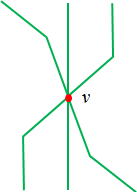
\includegraphics[width=0.2\textwidth]{figs/unrooted.png}
%  \caption{\label{fig:unrooted}%
%           An illustration of a tree skeleton that satisfies the angle constraint but is taken as two subgraphs by our algorithm.}
%\end{figure}

%However, we can evaluate the effectiveness of our approach by judging the topology of some simple models and evaluate how close our partition is from a potential optimal result. For example, from Figure \ref{fig:ex1}, under the requirement of $\theta = 70^{\circ}$, ignoring the tinny detailed geometric features we can observe that an optimal partition of the deer model requires at least $4$ cuts: the tail, the chunk including the legs, the neck, and the head and the horn. Our approach provides a partition of 4 cuts, which is almost near the optimal. Further, from the appearance of the gargoyle model (the last row of Figure \ref{fig:experiment}), we can see that an optimal cutting should have the following 4 parts: the head, two wings, and the remaining parts. Our partition results in 5 parts, which is very close to the potential optimal partition.

%Our approach is devoted to shell models, it can also be applied to cutting solid models without any problem. However, our approach suffers from a few limitations: for shell models, the thickness of the shells need to be large enough such that no serious deformation is caused during the assembling process. However, the problem of setting the minimum thickness of the model for various parts of the model is non-trivial, and our current work is restricted to a uniform setting of the shell thickness whose value is determined by an error-and-trial process. Further, the strength guarantee is not elaborated in this work, a possible solution is to use the algorithm in \cite{WangWYLTTDCL13} that distributes the least amount of materials for constructing a truss frame beneath the skin. Finally, our approach may allow a cut that passes through a salience region, which may hurt the appearance of the model. We found that it is difficult to make a balance between the saliency and the minimal cutting length as well as the minimal cutting numbers. A potential future research is to take care of salience region during graph partition. Finally, as a trade-off, a spatially curved cut might be a consideration to alleviate the salience problem.
